\chapter{Software}
\section{The software architecture}
The architecture of program is followed 3-tier model. There-tier architecture is an architecture that each tier is designed, developed and maintained as independent. The advantage of this architecture is intended to allow any upgraded or replaced independent between the tiers. When user want to change the requirements or technology of a tier, it will non-affect to other tiers.\\[0.3cm]
The architecture of three-tiers includes:
\begin{itemize}
	\item \textbf{Data tier}: includes the classes which were designed for the data structure of program. It also provides the persistence mechanism to access the data.
	\item \textbf{Logic tier}: controls the functionality of application by performing detailed processing.
	\item \textbf{Presentation tier}: displays information related to user. It is a layer which received the require from user to program or return the result from program to user. 
\end{itemize}
\begin{figure}[h]
	\centering
	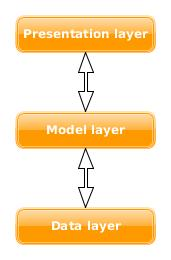
\includegraphics[scale=0.7]{images/software_3tiers}
	\caption{Three-tiers model}
	\label{fign3iters}
\end{figure}
\section{The modules}
The MAELab software mainly includes four modules: \textbf{segmentation}, \textbf{histograms}, \textbf{pht} and \textbf{correlation}. Besides, the software also includes the other modules to support for the main modules. The relation between the modules in the software is shown in figure \ref{fignsmodules}.
\begin{figure}[h]
	\centering
	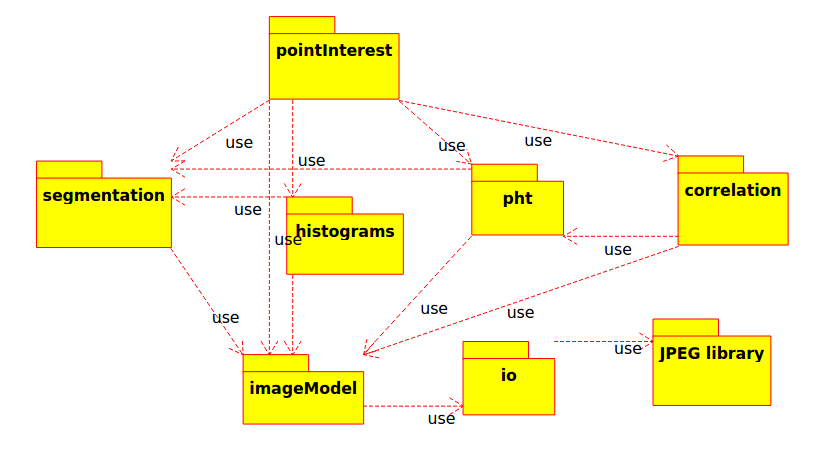
\includegraphics[scale=0.5]{images/modules}
	\caption{Three-tiers model}
	\label{fignsmodules}
\end{figure}
The functions of each modules is describing as followed:
\begin{itemize}
	\item \textbf{io} module: Implement the functions to read and write file. It includes the \textbf{JPEG library} that used to decode and encode the JPEG image.
	\item \textbf{imageModel} module: Represent the data structure of the image.
	\item \textbf{segmentation} module: Implement the segmentation methods on image.
	\item \textbf{histograms} module: Contains the methods to compute the geometric histogram of the image.
	\item \textbf{pht} module: Describe the probabilistic hough transform duration.
	\item \textbf{correlation} module: Includes the template matching methods.
	\item \textbf{pointInterest} module: Combine the result of the modules such as segementation, histograms,... to provide the adapter to other module or other software.
\end{itemize}
\section{The modules}
\section{The classes architecture}